\documentclass{article}
\usepackage{amsmath}
\usepackage{csquotes}
\usepackage{tikz}
\usepackage[a4paper]{geometry}
\usepackage{fancyhdr}
\pagestyle{fancy}
\lhead{Schwebung}
\rhead{September 2025}
\begin{document}
\section{Schwebung}
\begin{minipage}{\dimexpr\linewidth-6.5cm} 
Sind zwei schwingungsfähige Systeme gegeben, der Eigenfrequenzen $f_1$ und $f_2$ mit ${f_1 \approx f_2}$ aber ${f_1 \ne f_2}$, so kommt es bei einer Schwingung durch die Interferenz dazu, dass sich eine Welle bildet.
 
Die hier relevante Frequenz $f_S$ beschreibt nun die Einhüllende der neuen Schwingung. Sind beispielsweise beide Wellen Schallwellen, so beschreibt $f_S$ die Schwingung der Lautstärke. \par \vspace{2pt}
 
\end{minipage}
\hfill 
\begin{minipage}{5.5cm}
 \center
 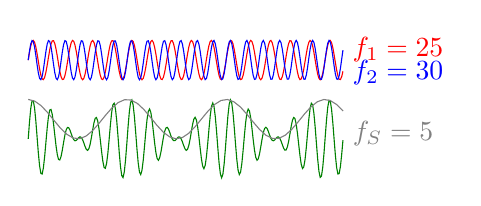
\begin{tikzpicture}
  \draw[red, domain=0:4, samples=250] plot (\x,{0.25*sin(25*\x r)}) node[above right] {$f_1=25$};
  \draw[blue, domain=0:4, samples=250] plot (\x,{0.25*sin(30*\x r)}) node[below right] {$f_2=30$};
 
  \draw[green!50!black, domain=0:4, samples=250] plot (\x,{(0.25*sin(25*\x r)+0.25*sin(30*\x r))-1}); 
  \draw[black!50, domain=0:4, samples=50] plot (\x,{(0.25*cos(5*\x r))-0.75}) node[below right] {$f_S=5$}; 
 \end{tikzpicture} 
\end{minipage}
 
\noindent Hier gilt
\[
 f_S = \vert f_1 - f_2 \vert
\] 
\end{document}